\section{Dataset description and operations}\label{sec:dataset}

In our work we employed the DEAM Dataset (\emph{MediaEval Database for Emotional Analysis in Music}) provided by the \emph{Swiss Center for Affective Sciences of the University of Geneva, Switzerland}.
The dataset consists of 2058 songs annotated with valence and arousal values, both continuously (per-second) and over the whole songs. Csv files containing features extracted from every song are also provided.

In particular, our work was focused, for the first 1744 songs, on the averaged static annotations of the dataset and on the features extracted from the music database. We used both the already provided features from the dataset and other features extracted ex novo.

\subsection{Music database}\label{sec:database}

The music database consists of royalty-free music from several sources: \textit{freemusicarchive.org} (FMA), \textit{jamendo.com}, and the \textit{medleyDB dataset}~\cite{bittner2014medleydb}. There are 1,744 clips of 45 seconds from FMA and 58 full length songs, half of which come from medleyDB and another half from Jamendo~\cite{aljanaki2017developing}.
The provided 45 seconds excerpts have all been re-encoded to have the same sampling frequency (i.e, 44.1\,kHz) and have been extracted from a random (uniformly distributed) starting point for any given song. Both the 45 seconds clips and full songs are provided in MPEG layer 3 (MP3) format~\cite{soleymani2016deam}.

The music from the FMA is in rock, pop, soul, blues, electronic, classical, hip-hop, international, experimental, folk, jazz, country and pop genres. The music from the MedleyDB dataset, in addition, has music in world and rap genres, and the music from Jamendo also has reggae music. For 2014 and 2015 data set, each song has been manually checked and the files with bad recording quality or those containing speech or noise instead of music have been excluded. For each artist, no more than 5 songs have been selected to be included in the dataset. For medleyDB and Jamendo full-length songs, only songs which had emotional variation in them have been selected, using an existing dynamic MER algorithm for filtering them and doing a final manual selection~\cite{anna2015emotion}.


\subsection{Annotations}\label{sec:annotations}

The dataset from 2013 and 2014 contains annotations on 45 seconds excerpts extracted from random points in songs. Each excerpt was annotated by a minimum of 10 workers and the static annotations were made on nine-point scale on valence and arousal for the whole 45 seconds excerpts~\cite{aljanaki2017developing}.
Then, averaged annotations have been generated with 2\,Hz sampling rate, providing both mean and standard deviation values~\cite{soleymani2016deam}.

We standardized annotations using the sklearn~\cite{scikit-learn} \texttt{scale} function of the \texttt{preprocessing} module, which centers the values around zero to eliminate the effects of possible anomalies. Table~\ref{table:annot-ranges} reports obtained ranges for each annotation after the standardization.

\begin{table}[h]
	\centering
	\begin{tabular}{cccc}
		\toprule
		valence mean & valence std & arousal mean & arousal std \\
		\midrule
		5.794 & 6.746 & 5.043 & 5.802 \\
		\bottomrule
	\end{tabular}
	\caption{Range (i.e. max-min) for each annotation after the standardization}
	\label{table:annot-ranges}
\end{table}


\subsection{Features}\label{sec:features}

A set of features extracted by \emph{openSMILE}~\cite{opensmile} for 500\,ms windows is provided with the dataset. We also extracted a set of additional features from the 45 seconds song excerpts using \emph{Librosa}~\cite{librosa}, computing for the latter 5 different statistical moments (mean, standard deviation, maximum, minimum and kurtosis).

We made several attempts in order to achieve best results in the cross-validation step (see section~\ref{sec:enhance-model}), so we first tried by separating tracks in two sets, a "high-annotation" set and a "low-annotation" set, for both valence and arousal mean/std values. Plotting the value distribution of a certain feature for some songs of each set, we could check if some differences were arising in the way those distributions gathered (e.g. see figure~\ref{fig:va_mean-spectral_flatness-dists}).

\begin{figure}
	\centering
	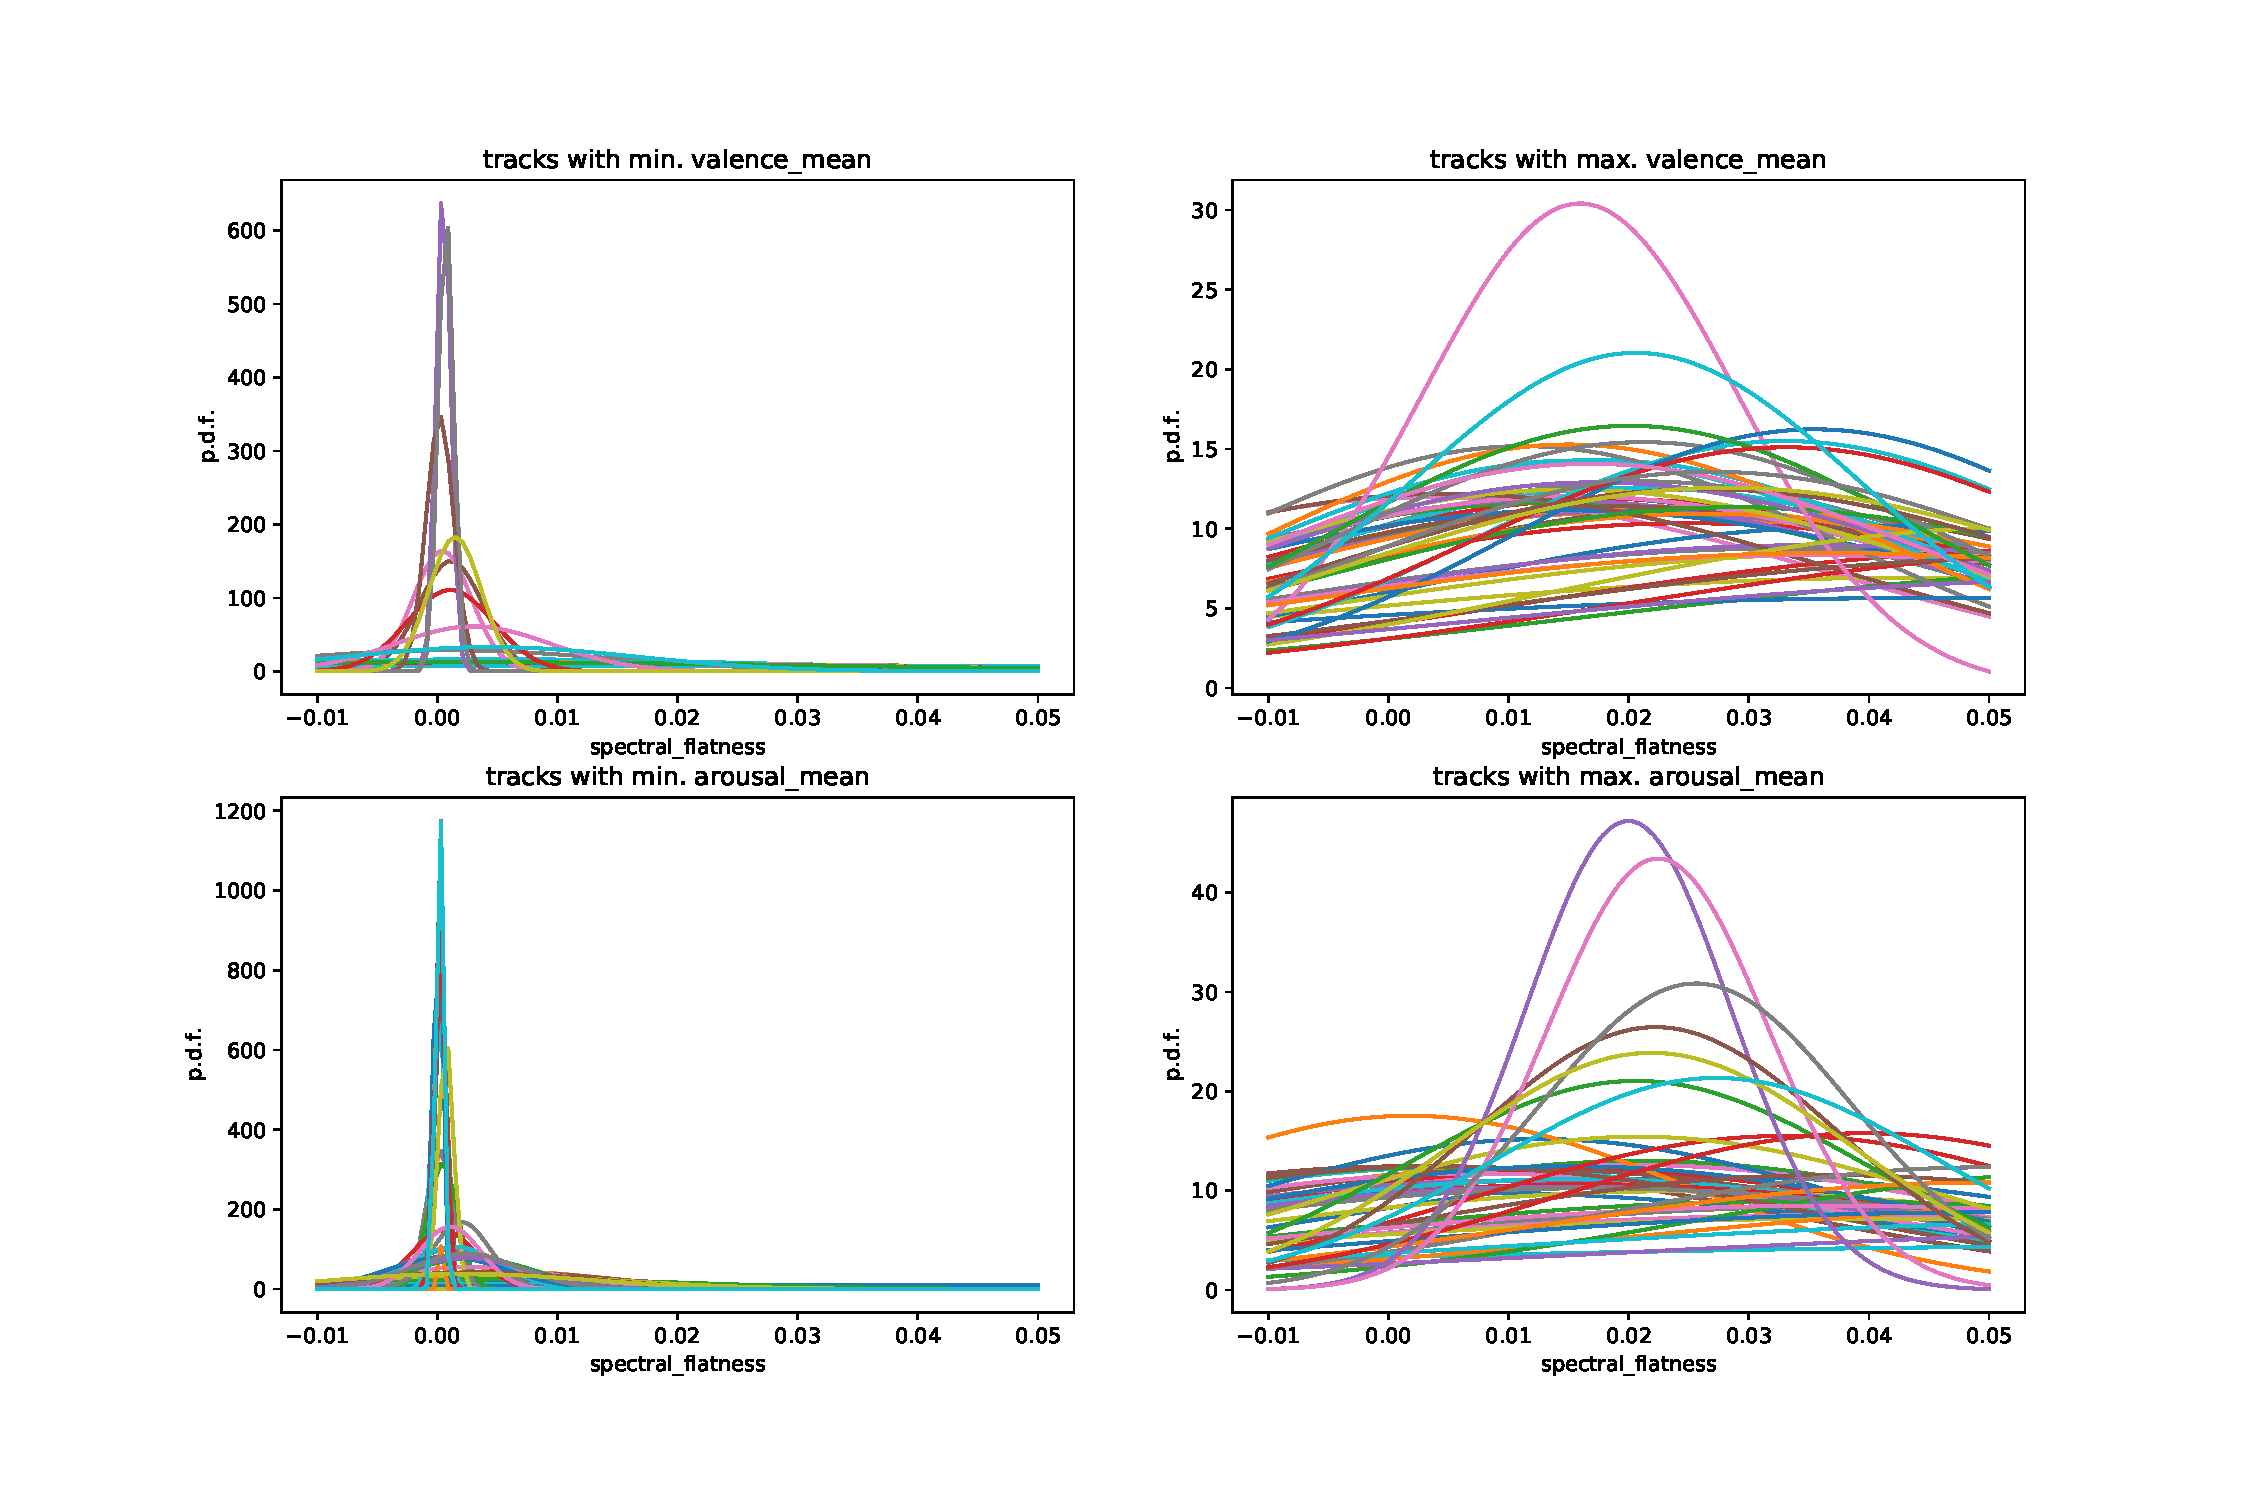
\includegraphics[width=\linewidth]{assets/va_mean-spectral_flatness-dists.pdf}
	\caption{Spectral flatness distribution}
	\label{fig:va_mean-spectral_flatness-dists}
\end{figure}

Then, we realized that a better way to visualize features might have been to plot feature-vs-annotation scatters (e.g. see figure~\ref{fig:scatter-spectral_bandwidth_amean}). This way, we could notice several linear relationships between a feature and the respective valence and/or arousal values. We used these results to make a preliminary manual feature selection. In particular we selected different features depending on the annotation to be predicted and discarded unneeded features.

\begin{figure}
	\centering
	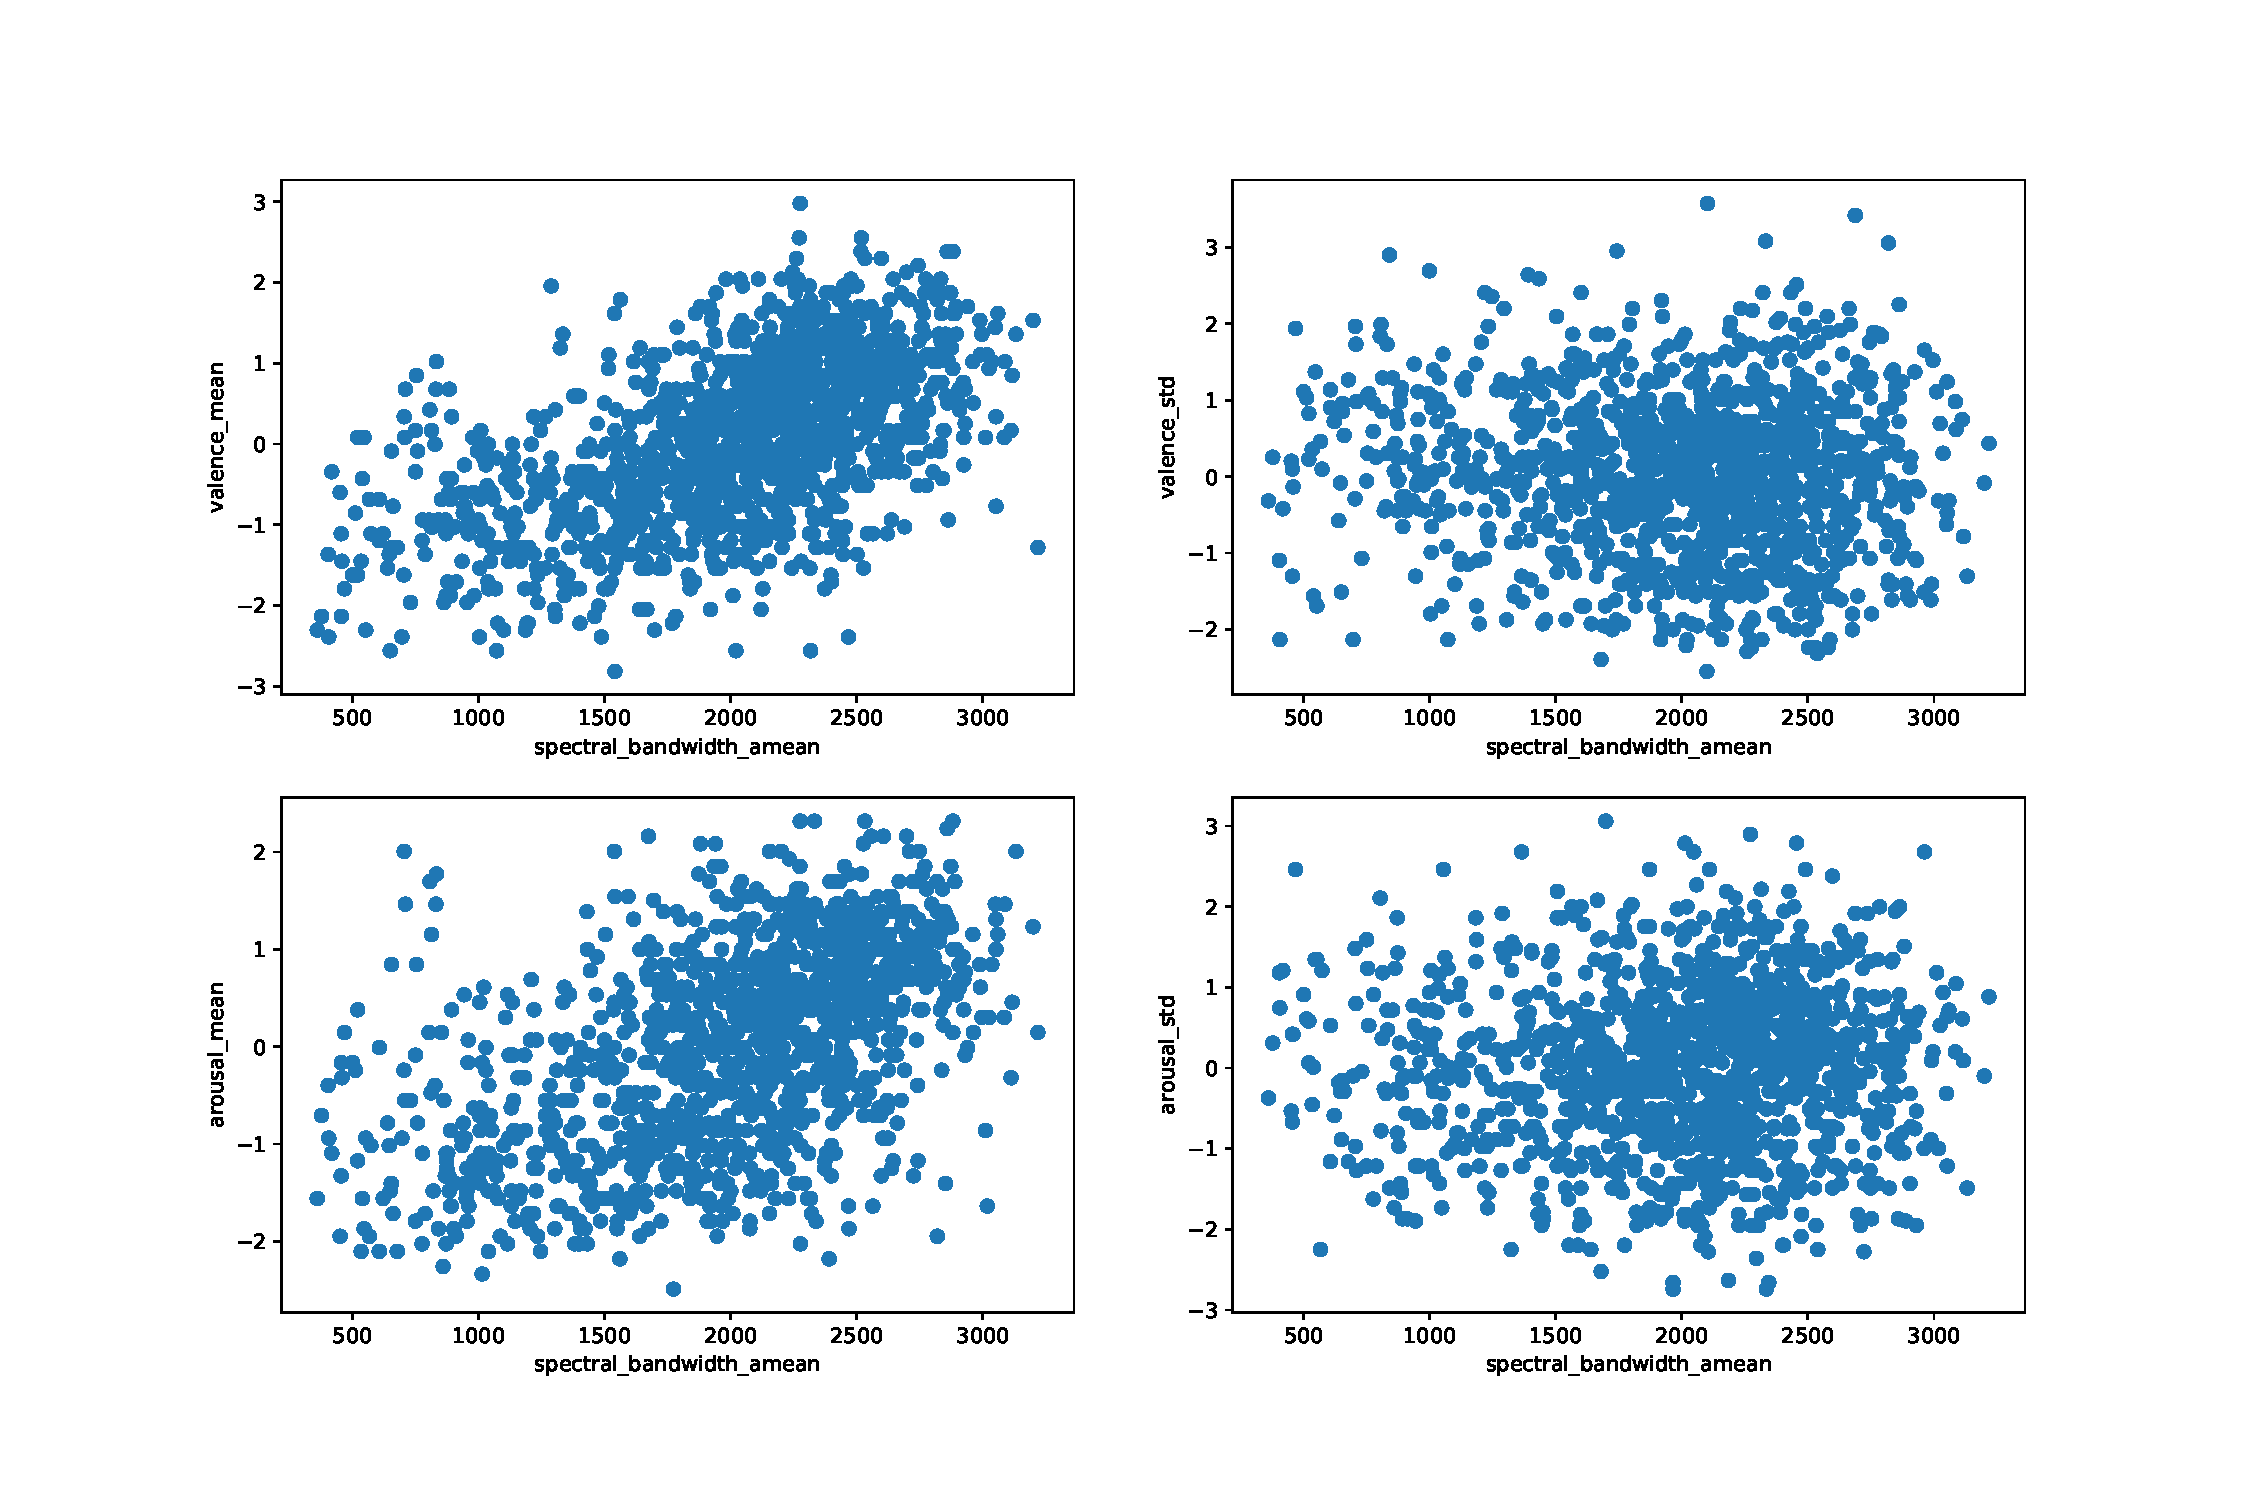
\includegraphics[width=\linewidth]{assets/scatter-spectral_bandwidth_amean.pdf}
	\caption{Spectral Bandwidth vs. Annotations scatter plot}
	\label{fig:scatter-spectral_bandwidth_amean}
\end{figure}

Finally, in addition to manual selection, we filter out unneeded or redundant features using automatic feature selection tools provided by sklearn, like ``recursive feature elimination'', ``select $k$-best'' and ``variance threshold''. In particular, the last two turned out to be the most effective.

For convenience, we arranged each feature processing step, including a standardization scaling (needed for some types of regressors, see section~\ref{sec:regression}), in a sklearn \texttt{Pipeline} that is executed before each fitting stage and predicting stage of the regressors.